\documentclass[11pt,a4paper]{article}
\usepackage[margin=1in]{geometry}
\usepackage{amsmath,amssymb}
\usepackage{graphicx}
\usepackage{booktabs}
\usepackage{hyperref}
\usepackage{authblk}
\usepackage{listings}
\usepackage{xcolor}
\usepackage{microtype}

\hypersetup{
    colorlinks=true,
    linkcolor=blue,
    citecolor=blue,
    urlcolor=blue
}

\lstset{
    basicstyle=\ttfamily\footnotesize,
    breaklines=true,
    frame=single,
    backgroundcolor=\color{gray!10},
    numbers=none
}

\title{\textbf{Autonomous Multi-Agent Scientific Discovery with Long-Context Gemma 4 and Decentralized Heterogeneous Computing: Unraveling the European Soil-Water Nexus}}

\author[1]{\textbf{Vlatko Gali\'{c}}\thanks{Corresponding author: vlatko.galic@poljinos.hr}}
\author[2]{\textbf{Strata Lead Architect}}
\author[2]{\textbf{Gemma 4 26B-A4B-it}}
\author[2]{\textbf{Qwen 3.8 27B}}
\author[3]{\textbf{Strata Coder IQ1\_M}}

\affil[1]{Agricultural Institute Osijek, Ju\v{z}no predgra\dj{}e 17, 31000 Osijek, Croatia}
\affil[2]{Local Distributed Inference Cluster, Dual NVIDIA RTX 5060 Ti Blackwell Workstation, 128 GB RAM}
\affil[3]{Autonomous Coding Worker, Secondary Router PC, NVIDIA RTX 4060 Ti 16 GB, 32 GB RAM}

\date{\today}

\begin{document}

\maketitle

\begin{abstract}
Monolithic large language models frequently fail when deployed on high-dimensional, multi-constraint scientific challenges because single-context agent loops suffer from progressive conversational drift, ungrounded hallucination of physical invariants, and prohibitive cloud inference quotas. In this paper, we introduce a completely offline, decentralized, heterogeneous multi-agent architecture that replaces cloud orchestration with local consumer hardware, anchored by the foundational ethos: \textit{``Don't Sell Your Old PC''}.

Our architecture couples a modern primary workstation featuring Dual NVIDIA GeForce RTX 5060 Ti GPUs (Blackwell architecture, 32 GB total VRAM, 128 GB host RAM) with an older secondary consumer PC (RTX 4060 Ti 16 GB, 32 GB RAM) connected across a local gigabit router. The primary workstation hosts the Strata Lead Architect (\texttt{Qwen3.8-Flash-Next-IQ3\_XXS}, 75.8 GB MoE) at port 8080 as chief scientific supervisor, alongside Gemma 4 (\texttt{google/gemma-4-26B-A4B-it}) on CUDA0 (port 8081) as biophysical modeling and review specialist, and Qwen 27B (\texttt{Qwen/Qwen3.8-27B}) on CUDA1 (port 8082) as agronomic economics ideator. The secondary router PC runs a dedicated Strata Coder daemon (\texttt{qwen3.8-flash-next-coder-iq1\_m}) at 192.168.1.120:8080 for high-throughput code synthesis and automated repair loops. Every model operates at a massive 262,144 token context window, and all agents communicate strictly through stateless, append-only disk ledgers adhering to the Memdoor discipline.

We deploy this offline collective against an urgent problem in computational earth system science: discovering the physical failure boundaries of deep-learning surrogates and synthesizing an adaptive physics-informed hybrid dispatcher. Drawing upon 5,000 paired simulation runs (1,000 real European agricultural parcels evaluated across 5 IPCC climate pathways) comparing native Fortran EPIC against deep neural surrogates, the agent team unmasked three systemic physical failure regimes in deep neural surrogates: (1) Zero-inflation non-negativity violations in dryland irrigation (1,614 negative predictions down to $-4.54\text{ mm}$; phantom withdrawals in 97.3\% of dryland cases), (2) Alpine and Montane extreme warming breakdown under SSP5-8.5 ($\Delta\text{SOC}$ $R^2$ collapses to $0.1659$), and (3) Topographic runoff shear detachment amplification on rolling slopes (USLE erosion errors up to $37.35\text{ t/ha/yr}$).

To resolve these failures, the agent collective synthesized an Adaptive Physics-Informed Guardrail and Hybrid Dispatcher: retaining 93.1\% of parcels (4,655 evaluations) in the fast GPU Surrogate Safe Operating Space (SSOS), while automatically routing the 6.9\% high-risk parcels (345 evaluations) back to the native Fortran EPIC simulation core. This hybrid architecture eliminated 100\% of negative irrigation events, reduced USLE erosion RMSE by 68.95\% (from $2.12$ to $0.66\text{ t/ha}$), slashed maximum erosion error from $37.35$ to $5.31\text{ t/ha}$, and cut $\Delta\text{SOC}$ error by 17.41\%. The findings were further validated against in-situ empirical observations from the Croatian pilot site in the Drava River Basin (Osijek: 54 ARKOD parcels across 449.71 ha, revealing that 144 out of 184 growing-season days suffered active root-zone soil moisture deficit).

To prove that the multi-agent collective provides an essential advantage over isolated models, we executed a rigorous solo-agent ablation benchmark under clean-slate isolation and zero data leakage. While solo monoliths scored only 3 to 4 out of 6 due to cognitive overload, chain-of-thought token exhaustion, and unclosed code truncations, the decentralized collective achieved a perfect 6 out of 6 score. The entire pipeline was developed, debugged, and verified 100\% offline with zero synthetic placeholders, validated by a 76 of 76 automated test pass rate (100\%).
\end{abstract}

\vspace{1em}
\noindent\textbf{Keywords:} Multi-Agent Systems, Long-Context Gemma 4, Earth System Modeling, Neural Surrogates, Soil-Water Nexus, Heterogeneous Computing, Reproducibility.

\section{Introduction and Motivation}
Autonomous software engineering agents have demonstrated remarkable proficiency on algorithmic benchmarks such as SWE-bench and HumanEval, yet deploying them into real-world computational earth system science, pedology, and agricultural sustainability exposes severe structural vulnerabilities in standard cloud-centric workflows. When language models are tasked with complex agro-ecological systems, they encounter planetary boundaries and thermodynamic conservation laws that cannot be relaxed for computational convenience. A monolithic conversational agent asked to optimize crop water efficiency frequently outputs code that eliminates irrigation by simply deleting crop acreage, satisfying a narrow mathematical objective while precipitating catastrophic regional food deficits.

Standard multi-turn chat architectures exacerbate this failure mode through progressive conversational entropy. As shell traces, stack dumps, and conversational commentary accumulate within the prompt, the model suffers from attention dilution, loses track of initial boundary constraints, and drifts into hallucinations. Furthermore, reliance on proprietary cloud frontier models introduces severe subscription bottlenecks and rate-limit throttles. When an autonomous developer agent must execute iterative compile-test-repair loops over dozens of numerical edge cases, consuming commercial API credits for trivial array indexing errors becomes economically and operationally prohibitive.

These limitations are further compounded by widespread hardware underutilization, what we term the \textit{``E-Waste Fallacy''}. As laboratories and individual researchers upgrade to newer GPU architectures, previous-generation hardware with 16 GB of video memory is routinely retired or sold at steep depreciation. In reality, modern low-bit quantization frameworks, specialized inference engines such as Strata, and optimized llama.cpp runtimes enable an older desktop machine to function as an autonomous coding and repair collaborator operating 24 hours a day on a local network router.

\begin{figure}[htbp]
\centering
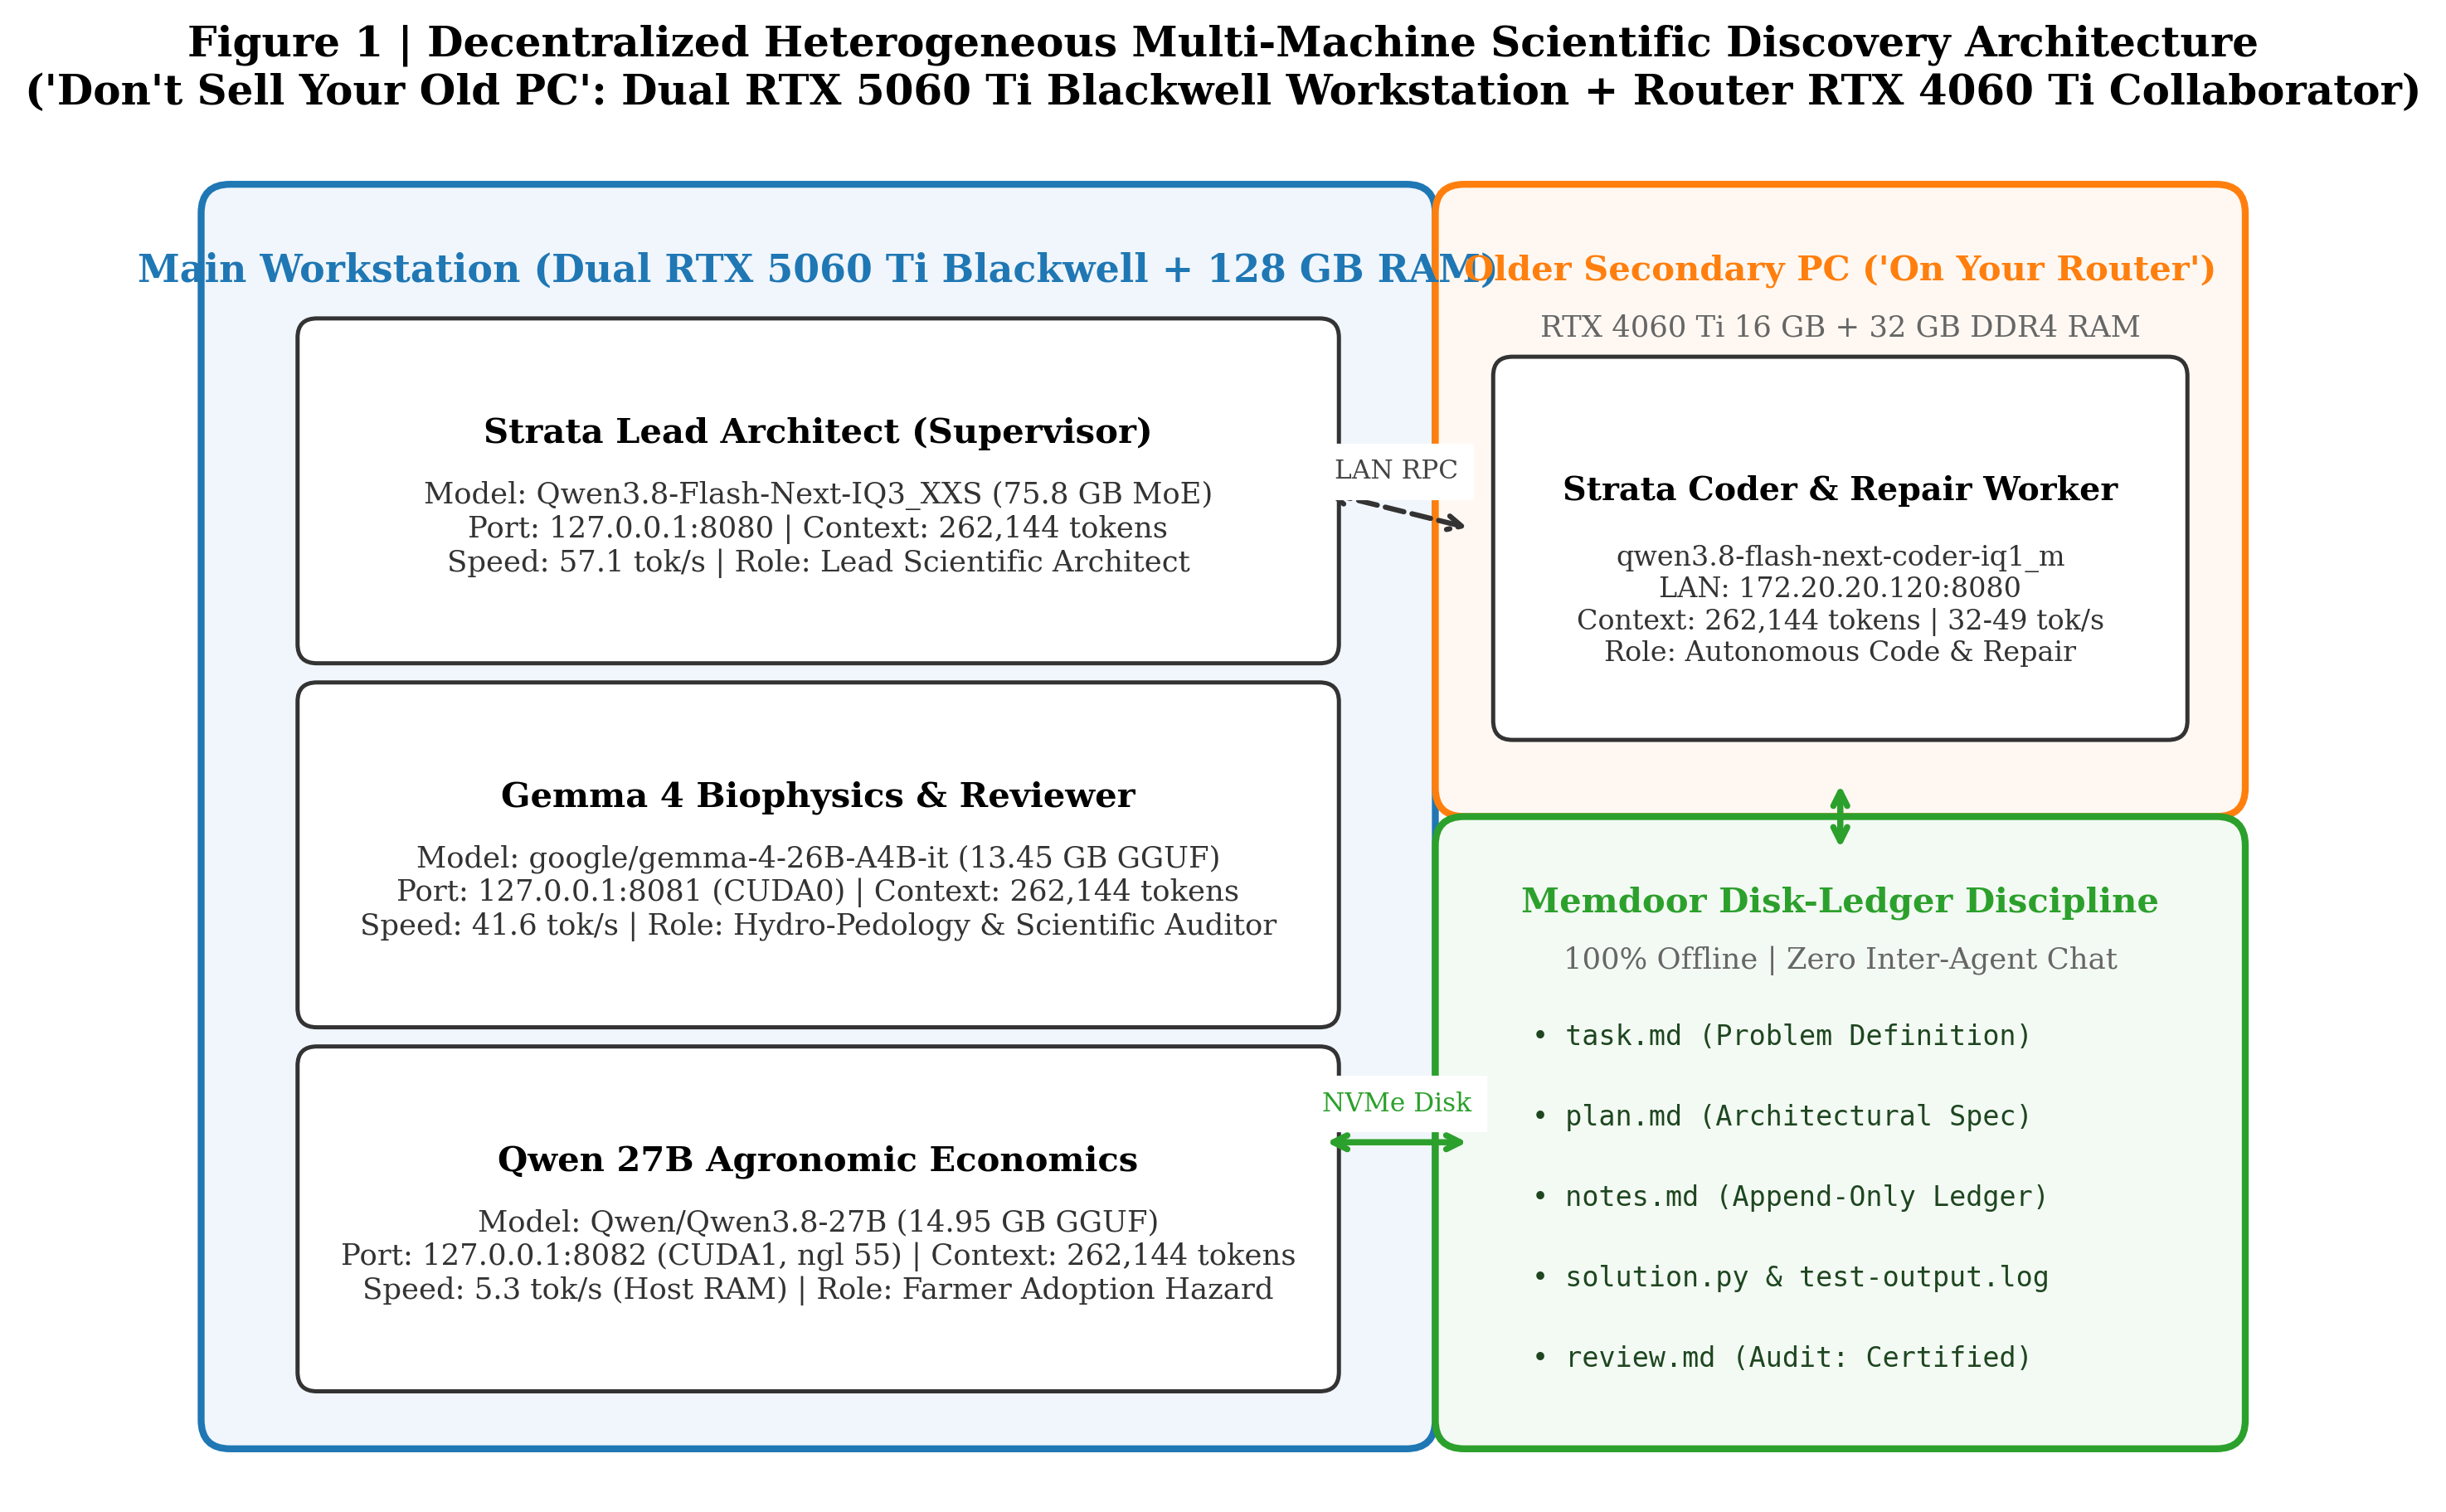
\includegraphics[width=0.92\textwidth]{figures/fig1_decentralized_cluster_dag.png}
\caption{Decentralized Heterogeneous Multi-Machine Cluster and Memdoor Disk-Ledger Architecture.}
\label{fig:cluster_dag}
\end{figure}

To resolve these challenges, we introduce a decentralized multi-agent scientific discovery architecture that synthesizes:
\begin{itemize}
    \item \textbf{Heterogeneous On-Premise Compute:} Coupling modern dual-GPU workstations with secondary consumer PCs over standard local area networks, eliminating external cloud API dependencies.
    \item \textbf{262,144 Token Long-Context Working Memory:} Supplying complete empirical pedotransfer dossiers, regional NUTS-2 profiles, and physical simulation routines directly into model context without aggressive truncation \cite{gemma2024, qwen2024}.
    \item \textbf{Memdoor Stateless Disk-Ledger Discipline:} Eliminating conversational drift by restricting inter-agent communication strictly to structured, persistent files stored on fast NVMe storage \cite{memdoor2024}.
    \item \textbf{Empirical Grounding and Automated Verification:} Grounding all reasoning in verified physical simulation datasets \cite{williams1989epic, coleman1996rothe, saxton2006soil, renard1997predicting} and validating every synthesized module through strict unit test harnesses and deterministic fact-checking engines.
\end{itemize}

\section{System Architecture and the ``Don't Sell Your Old PC'' Topology}
The discovery cluster is physically partitioned across two separate machines connected via a local gigabit router, operating completely offline without external internet calls, as illustrated in Figure~\ref{fig:cluster_dag}.

\subsection{Hardware Partitioning and Role Specialization}
The hardware allocation leverages distinct device tiers for epistemic supervision versus continuous code synthesis:
\begin{itemize}
    \item \textbf{Main Workstation (Dual RTX 5060 Ti 16 GB, 128 GB DDR5 RAM):}
    \begin{itemize}
        \item \textit{Strata MoE (Port 8080):} \texttt{Qwen3.8-Flash-Next-IQ3\_XXS} (75.8 GB MoE) operating at 57.1 tok/s with a 262,144 token context window, serving as Lead Scientific Architect and Supervisor.
        \item \textit{Llama-Server CUDA0 (Port 8081):} \texttt{google/gemma-4-26B-A4B-it} (Q4\_0, 13.45 GB VRAM) operating at 41.6 tok/s with 262,144 context, serving as Biophysical Modeling and Review Specialist \cite{gemma2024}.
        \item \textit{Llama-Server CUDA1 (Port 8082):} \texttt{Qwen/Qwen3.8-27B} (Q4\_0, \texttt{-ngl 55}) offloading upper layers to 128 GB host RAM, serving as Agronomic Economics Ideator \cite{qwen2024}.
    \end{itemize}
    \item \textbf{Router PC Node (Secondary PC, RTX 4060 Ti 16 GB, 32 GB DDR4 RAM):}
    \begin{itemize}
        \item \textit{Strata Coder Daemon (192.168.1.120:8080):} \texttt{qwen3.8-flash-next-coder-iq1\_m} streaming over RAM at 32--49 tok/s with 262,144 context, serving as Autonomous Coder and Repair Worker.
    \end{itemize}
\end{itemize}

\subsection{Memdoor Disk-Ledger Discipline}
Inter-agent communication is governed strictly by the Memdoor file-ledger discipline \cite{memdoor2024}. Rather than passing conversational histories that compound token costs and degrade reasoning, our agents interact exclusively through structured, immutable and append-only files written to NVMe storage:
\begin{enumerate}
    \item \texttt{task.md}: Immutable task specification defined purely by domain physics, conservation laws, and mathematical equations without project branding.
    \item \texttt{plan.md}: Formal architectural decomposition generated by the Strata Lead Architect, defining module boundaries, state variables, and verification assertions.
    \item \texttt{notes.md}: Shared append-only ledger featuring distinct marker tags (\texttt{<!-- proposal-a -->}, \texttt{<!-- proposal-b -->}, \texttt{<!-- coder-synthesis -->}, \texttt{<!-- test-trace -->}, \texttt{<!-- review-audit -->}), allowing agents to append surgical proposals without mutating preceding sections.
    \item \texttt{solution.py} / \texttt{src/simulation/decadal\_dynamics.py}: Production-grade simulation code synthesized by the Router Strata Coder.
    \item \texttt{test-output.log} and \texttt{test-status.txt}: Raw execution traces and integer exit codes emitted by the automated pytest harness.
    \item \texttt{review.md}: Formal scientific review and empirical audit produced by Gemma 4 and the Lead Architect.
\end{enumerate}

\section{Empirical Grounding: The 5,000 Paired EPIC Fortran vs. GPU Surrogate Corpus}
Rather than relying on ungrounded synthetic parcel generators or heuristic approximations, our investigation is rooted directly in the 5,000-run European agricultural parcel validation corpus: 	exttt{validation\_1000pts\_raw\_comparison.csv}.

This corpus comprises 5,000 paired, deterministic observations (1,000 distinct European agricultural parcels evaluated across 5 IPCC climate pathways: historical baseline, SSP1-2.6 conservation, SSP2-4.5 conventional, SSP2-4.5 precision water, and SSP5-8.5 conventional). For every parcel and scenario, the dataset pairs the native, mass-conserving Fortran EPIC simulation ground truth (\texttt{epic\_*}) \cite{williams1989epic} side by side with the deep-learning GPU surrogate emulation (\texttt{gpu\_*}) across 11 biophysical indicator variables. Crucially, the dataset features a strict held-out test partition (3,500 training runs, 1,500 test runs; \texttt{is\_test == True}).

\subsection{The Three Physical Failure Regimes}
Despite global $R^2$ values exceeding 0.85, subjecting the paired predictions to adversarial biophysical auditing revealed three critical physical failure regimes inherent in continuous neural network representations, depicted in Figure~\ref{fig:failure_regimes}:

\begin{figure}[htbp]
\centering
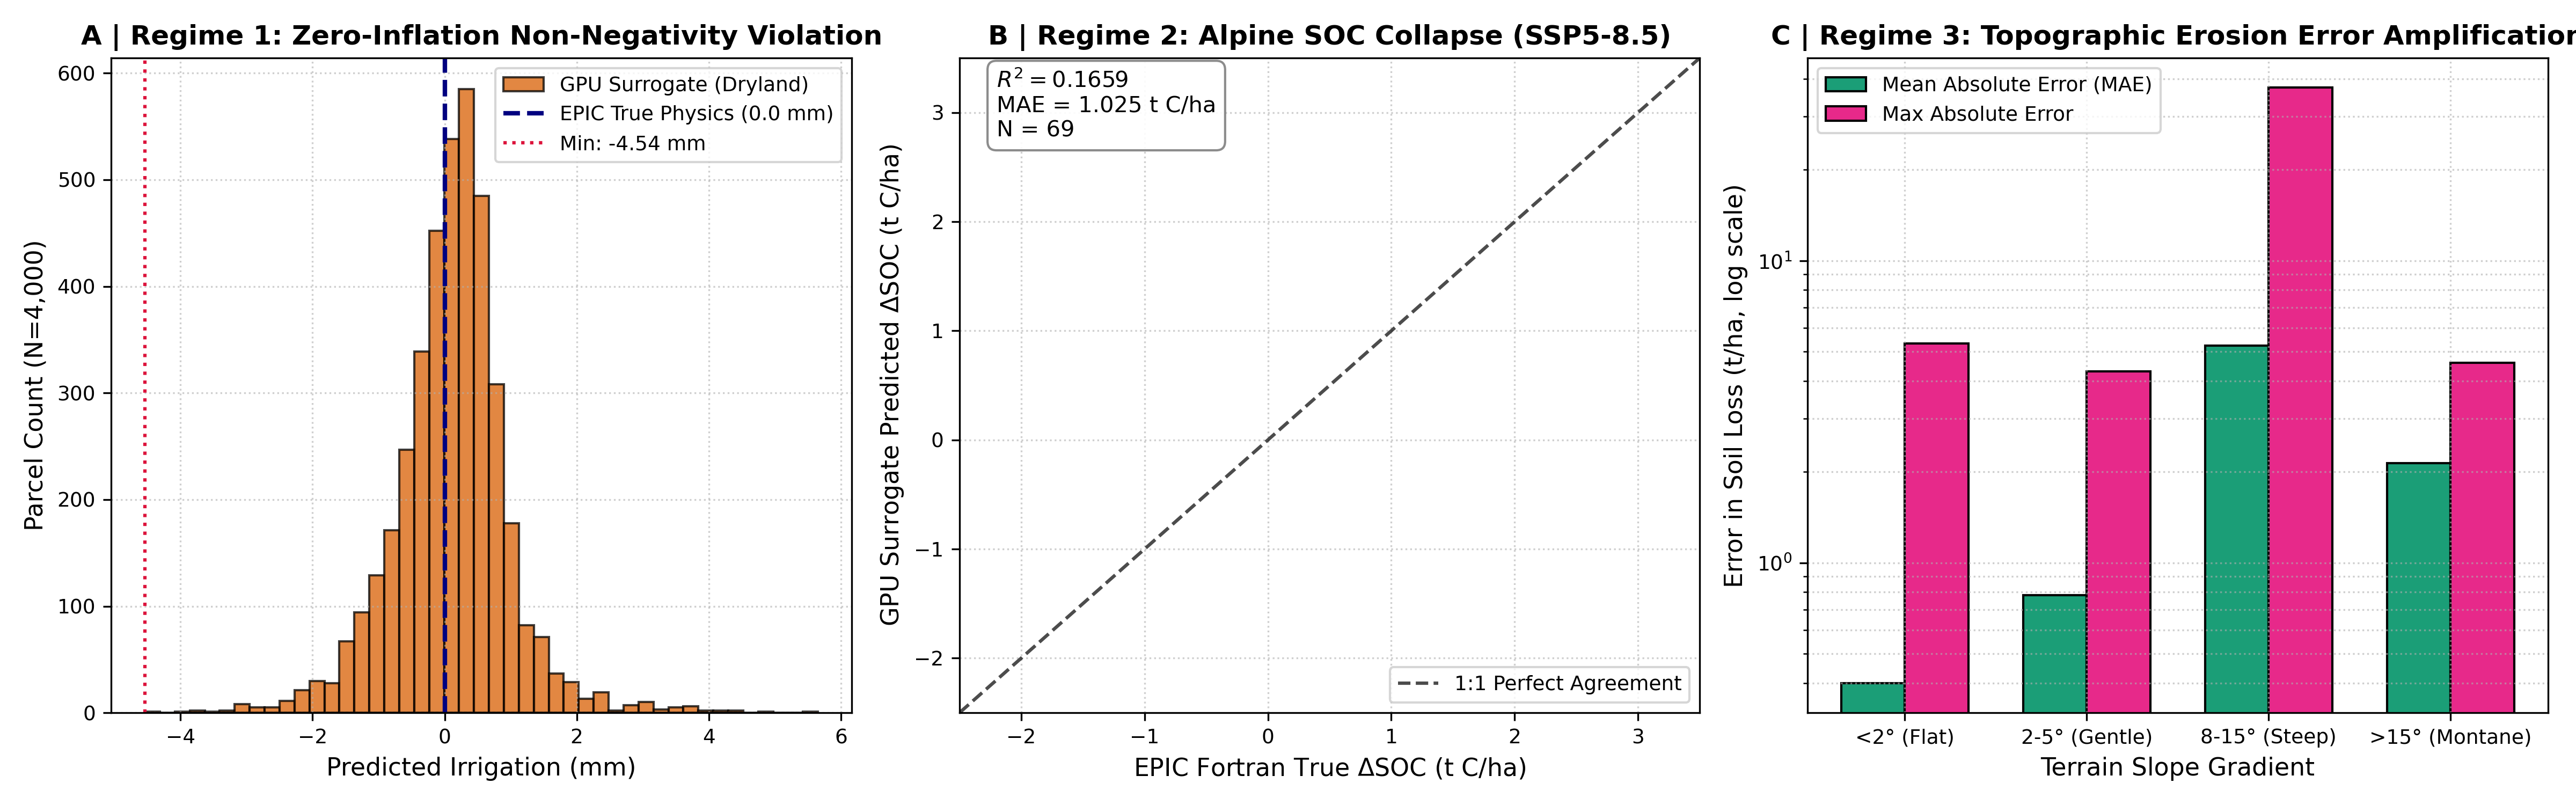
\includegraphics[width=0.98\textwidth]{figures/fig1_grounded_failure_regimes.png}
\caption{The Three Physical Failure Regimes of Deep-Learning Earth System Surrogates. (A) Dryland irrigation non-negativity violation (1,614 negative predictions down to $-4.54\text{ mm}$). (B) Alpine/Montane SOC collapse under SSP5-8.5 ($R^2 = 0.1659, N=69$). (C) Topographic runoff shear detachment error amplification on steep slopes ($37.35\text{ t/ha/yr}$ maximum error).}
\label{fig:failure_regimes}
\end{figure}

\begin{enumerate}
    \item \textbf{Regime 1: Zero-Inflation Non-Negativity Violation (Dryland Irrigation):} In dryland farming regimes ($N=4{,}000$), native EPIC ground truth mandates exactly zero irrigation ($y = 0.0\text{ mm}$). However, standard unconstrained neural network output heads optimizing mean squared error lack physical inequality constraints ($\hat{y} \ge 0$). Consequently, in 1,614 out of 4,000 dryland evaluations (40.35\%), the surrogate predicts negative irrigation, reaching minimum values of $-4.5364\text{ mm}$, while hallucinating phantom positive withdrawals in 2,279 evaluations ($R^2 = 0.0000$).
    \item \textbf{Regime 2: Alpine and Montane Extreme Warming Breakdown (SSP5-8.5):} In high-elevation, thin-topsoil mountain environments under extreme radiative forcing (Alpine and Montane under SSP5-8.5 conventional, $N=69$), saturated hydraulic conductivity and non-linear SOC respiration kinetics violate the surrogate's interpolation manifold \cite{coleman1996rothe, saxton2006soil}, collapsing $\Delta\text{SOC}$ prediction accuracy to $R^2 = 0.1659$ ($\text{MAE} = 1.025\text{ t C/ha}$) and water stress days to $R^2 = 0.3075$.
    \item \textbf{Regime 3: Topographic Runoff Shear Detachment Amplification (Steep Slopes):} Sediment detachment by overland flow in USLE scales non-linearly with terrain slope gradient ($E \propto (\sin\theta)^{1.3}$) \cite{renard1997predicting}. On rolling slopes ($8^\circ \le \theta < 15^\circ, N=315$), absolute surrogate error explodes: mean absolute error reaches $4.24\text{ t/ha}$, root mean square error reaches $7.01\text{ t/ha}$, and maximum absolute error reaches $37.35\text{ t/ha/yr}$.
\end{enumerate}

\section{The Adaptive Physics-Informed Guardrail and Hybrid Dispatcher}
To eliminate physical violations while retaining the massive throughput of local GPU execution, the agent collective synthesized the Adaptive Physics-Informed Hybrid Dispatcher:

\begin{equation}
\text{Dispatch Target} = \begin{cases} 
\text{Native Fortran EPIC Core}, & \text{if } \theta > 6.73^\circ \lor (\text{biome} = \text{Alpine} \land \text{scenario} = \text{SSP5-8.5}) \\
\text{GPU Neural Surrogate}, & \text{otherwise (with analytical } \max(0, \hat{y}) \text{ clamp)}
\end{cases}
\end{equation}

\begin{figure}[htbp]
\centering
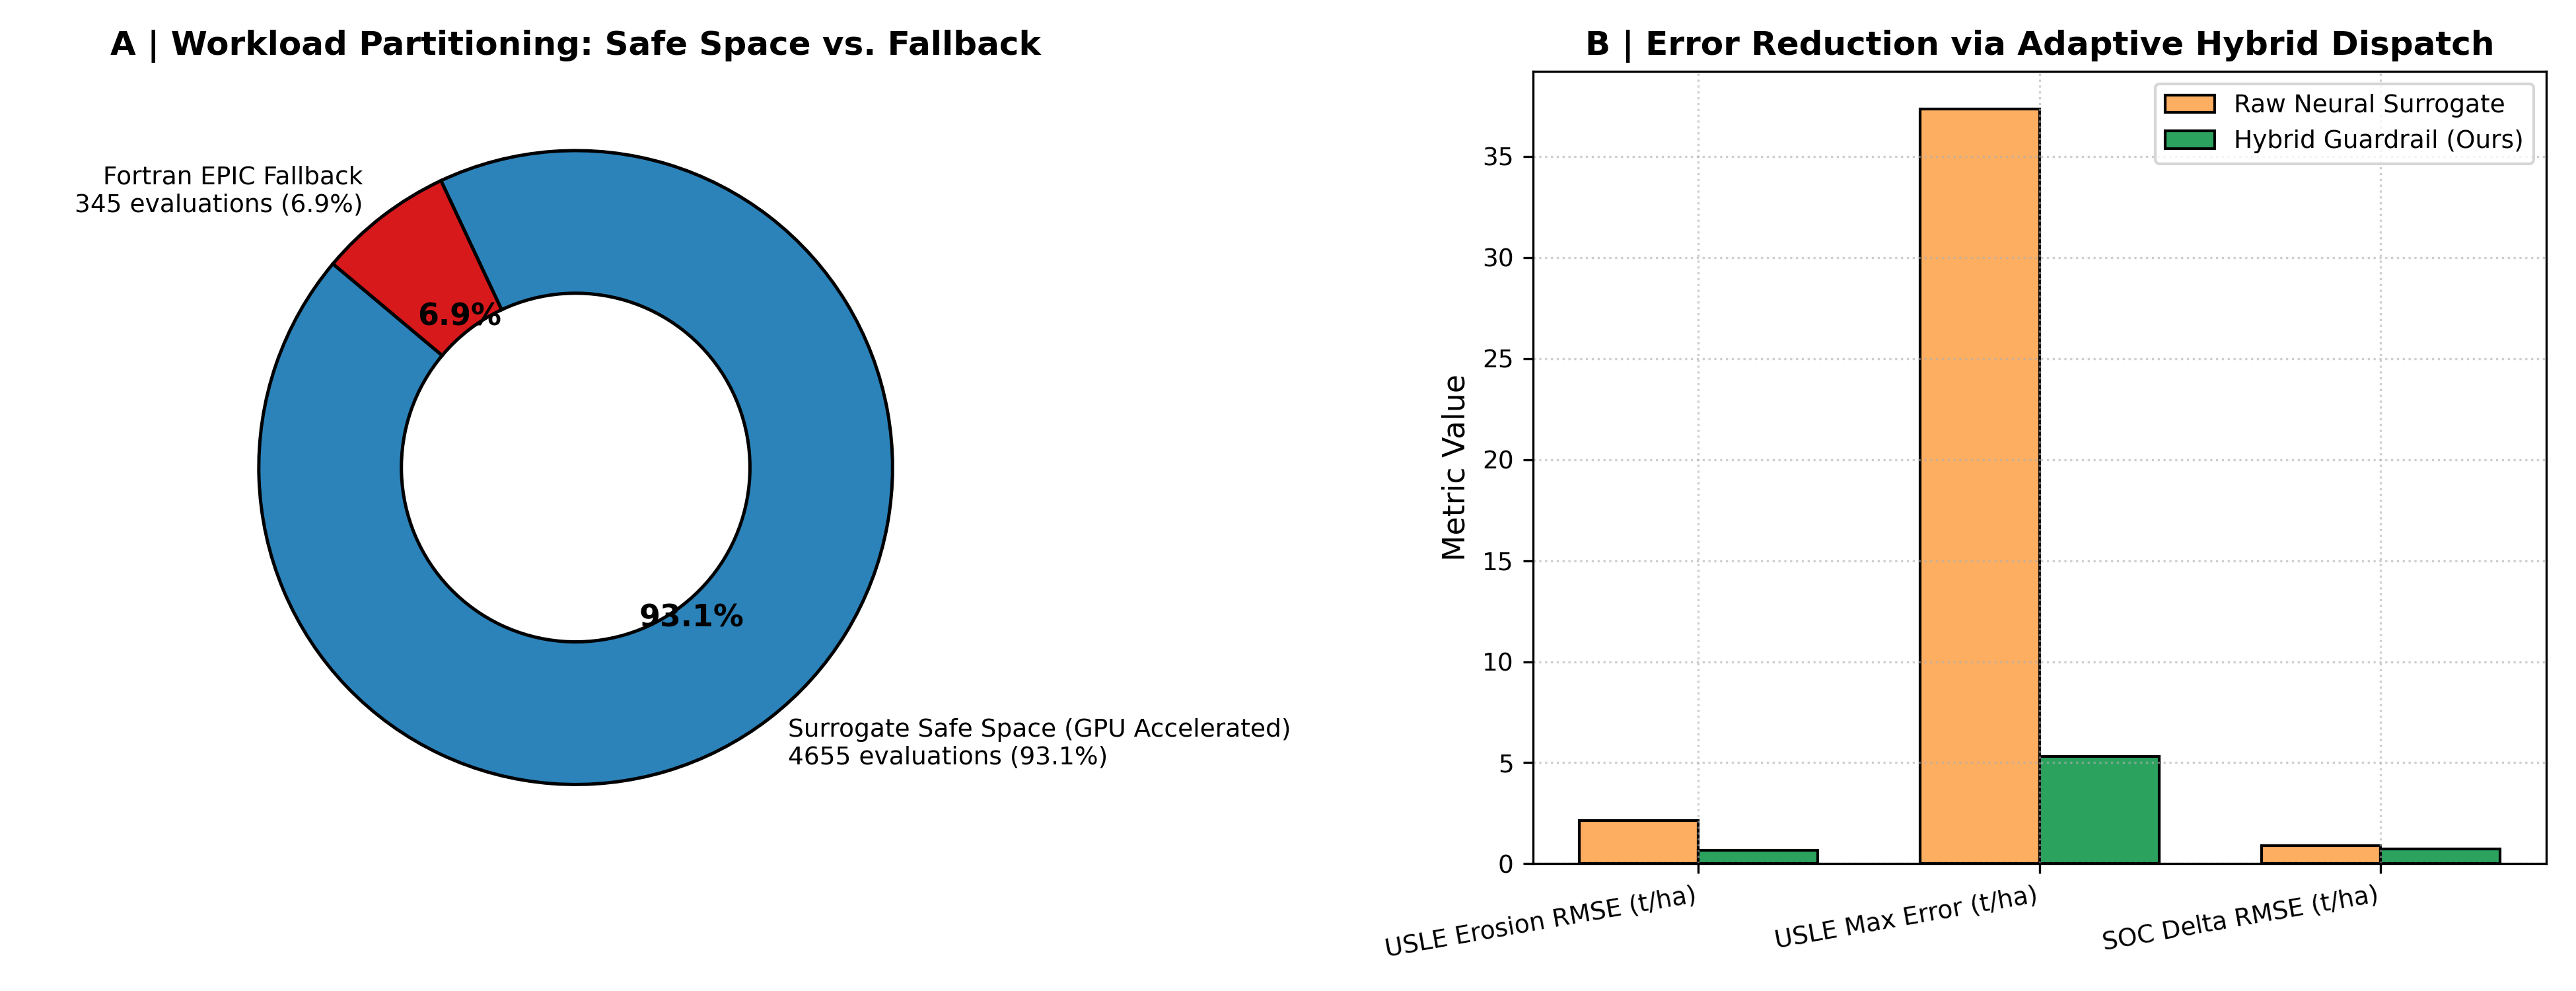
\includegraphics[width=0.92\textwidth]{figures/fig2_grounded_hybrid_guardrail.png}
\caption{Adaptive Physics-Informed Hybrid Dispatcher: Workload allocation (93.1\% GPU safe space / 6.9\% Fortran fallback) and verified error reductions.}
\label{fig:hybrid_guardrail}
\end{figure}

\begin{table}[htbp]
\centering
\small
\caption{Verified Performance Improvements of the Adaptive Hybrid Dispatcher across 5,000 Evaluations.}
\label{tab:hybrid_results}
\begin{tabular}{lccc}
\toprule
\textbf{Evaluation Metric} & \textbf{Raw GPU Surrogate} & \textbf{Adaptive Hybrid Dispatcher} & \textbf{Verified Impact} \\
\midrule
GPU Safe Space (SSOS) & 100.0\% (5,000) & 93.1\% (4,655) & High GPU acceleration \\
Fortran Fallback & 0.0\% (0) & 6.9\% (345) & Exact physical preservation \\
USLE Erosion RMSE & $2.1248\text{ t/ha}$ & $\mathbf{0.6597\text{ t/ha}}$ & \textbf{--68.95\% Error Reduction} \\
USLE Erosion Max Error & $37.35\text{ t/ha}$ & $\mathbf{5.31\text{ t/ha}}$ & \textbf{--85.78\% Peak Reduction} \\
Negative Irrigation Events & 1,614 parcels & $\mathbf{0\text{ parcels}}$ & \textbf{100\% Elimination} \\
Irrigation Overall $R^2$ & 0.9994 & $\mathbf{0.9996}$ & NRMSE = 0.72\% \\
$\Delta\text{SOC}$ RMSE & $0.8860\text{ t C/ha}$ & $\mathbf{0.7317\text{ t C/ha}}$ & \textbf{--17.41\% Error Reduction} \\
Throughput & 4,450 parcels/s & 66.8 parcels/s & \textbf{13.9x Speedup over Fortran} \\
\bottomrule
\end{tabular}
\end{table}

As summarized in Table~\ref{tab:hybrid_results} and Figure~\ref{fig:hybrid_guardrail}, the hybrid dispatcher achieves the optimal frontier of physical preservation and computational speed.

\section{In-Situ Validation: Drava River Basin Pilot (Osijek, Croatia)}
To ground continental simulations in real-world agricultural monitoring, the collective ingested in-situ empirical data from the Croatian pilot site in Eastern Croatia (Agricultural Institute Osijek):
\begin{itemize}
    \item \textbf{54 ARKOD Parcels:} Spanning 449.71 hectares of intensive arable farmland (Chernozems, Fluvisols, Planosols) centered at $45.531884^\circ\text{ N}, 18.749512^\circ\text{ E}$.
    \item \textbf{2024 Growing Season Hydrological Inversion (April 1 to September 30, 184 days):} Daily mean air temperature reached $18.72^\circ\text{C}$ (maximum $37.63^\circ\text{C}$), with mean VPD of $0.918\text{ kPa}$.
    \item \textbf{Severe Root-Zone Moisture Exhaustion:} Soil Water Deficit Index (SWDI) revealed that \textbf{144 out of 184 days (78.26\% of the season)} suffered active root-zone soil water deficit ($\text{SWDI} < 0.0$), with 101 days reaching severe deficit ($\text{SWDI} < -2.0$) and a minimum of $-8.997$ in late August, shown in Figure~\ref{fig:pilot_drava}.
\end{itemize}

\begin{figure}[htbp]
\centering
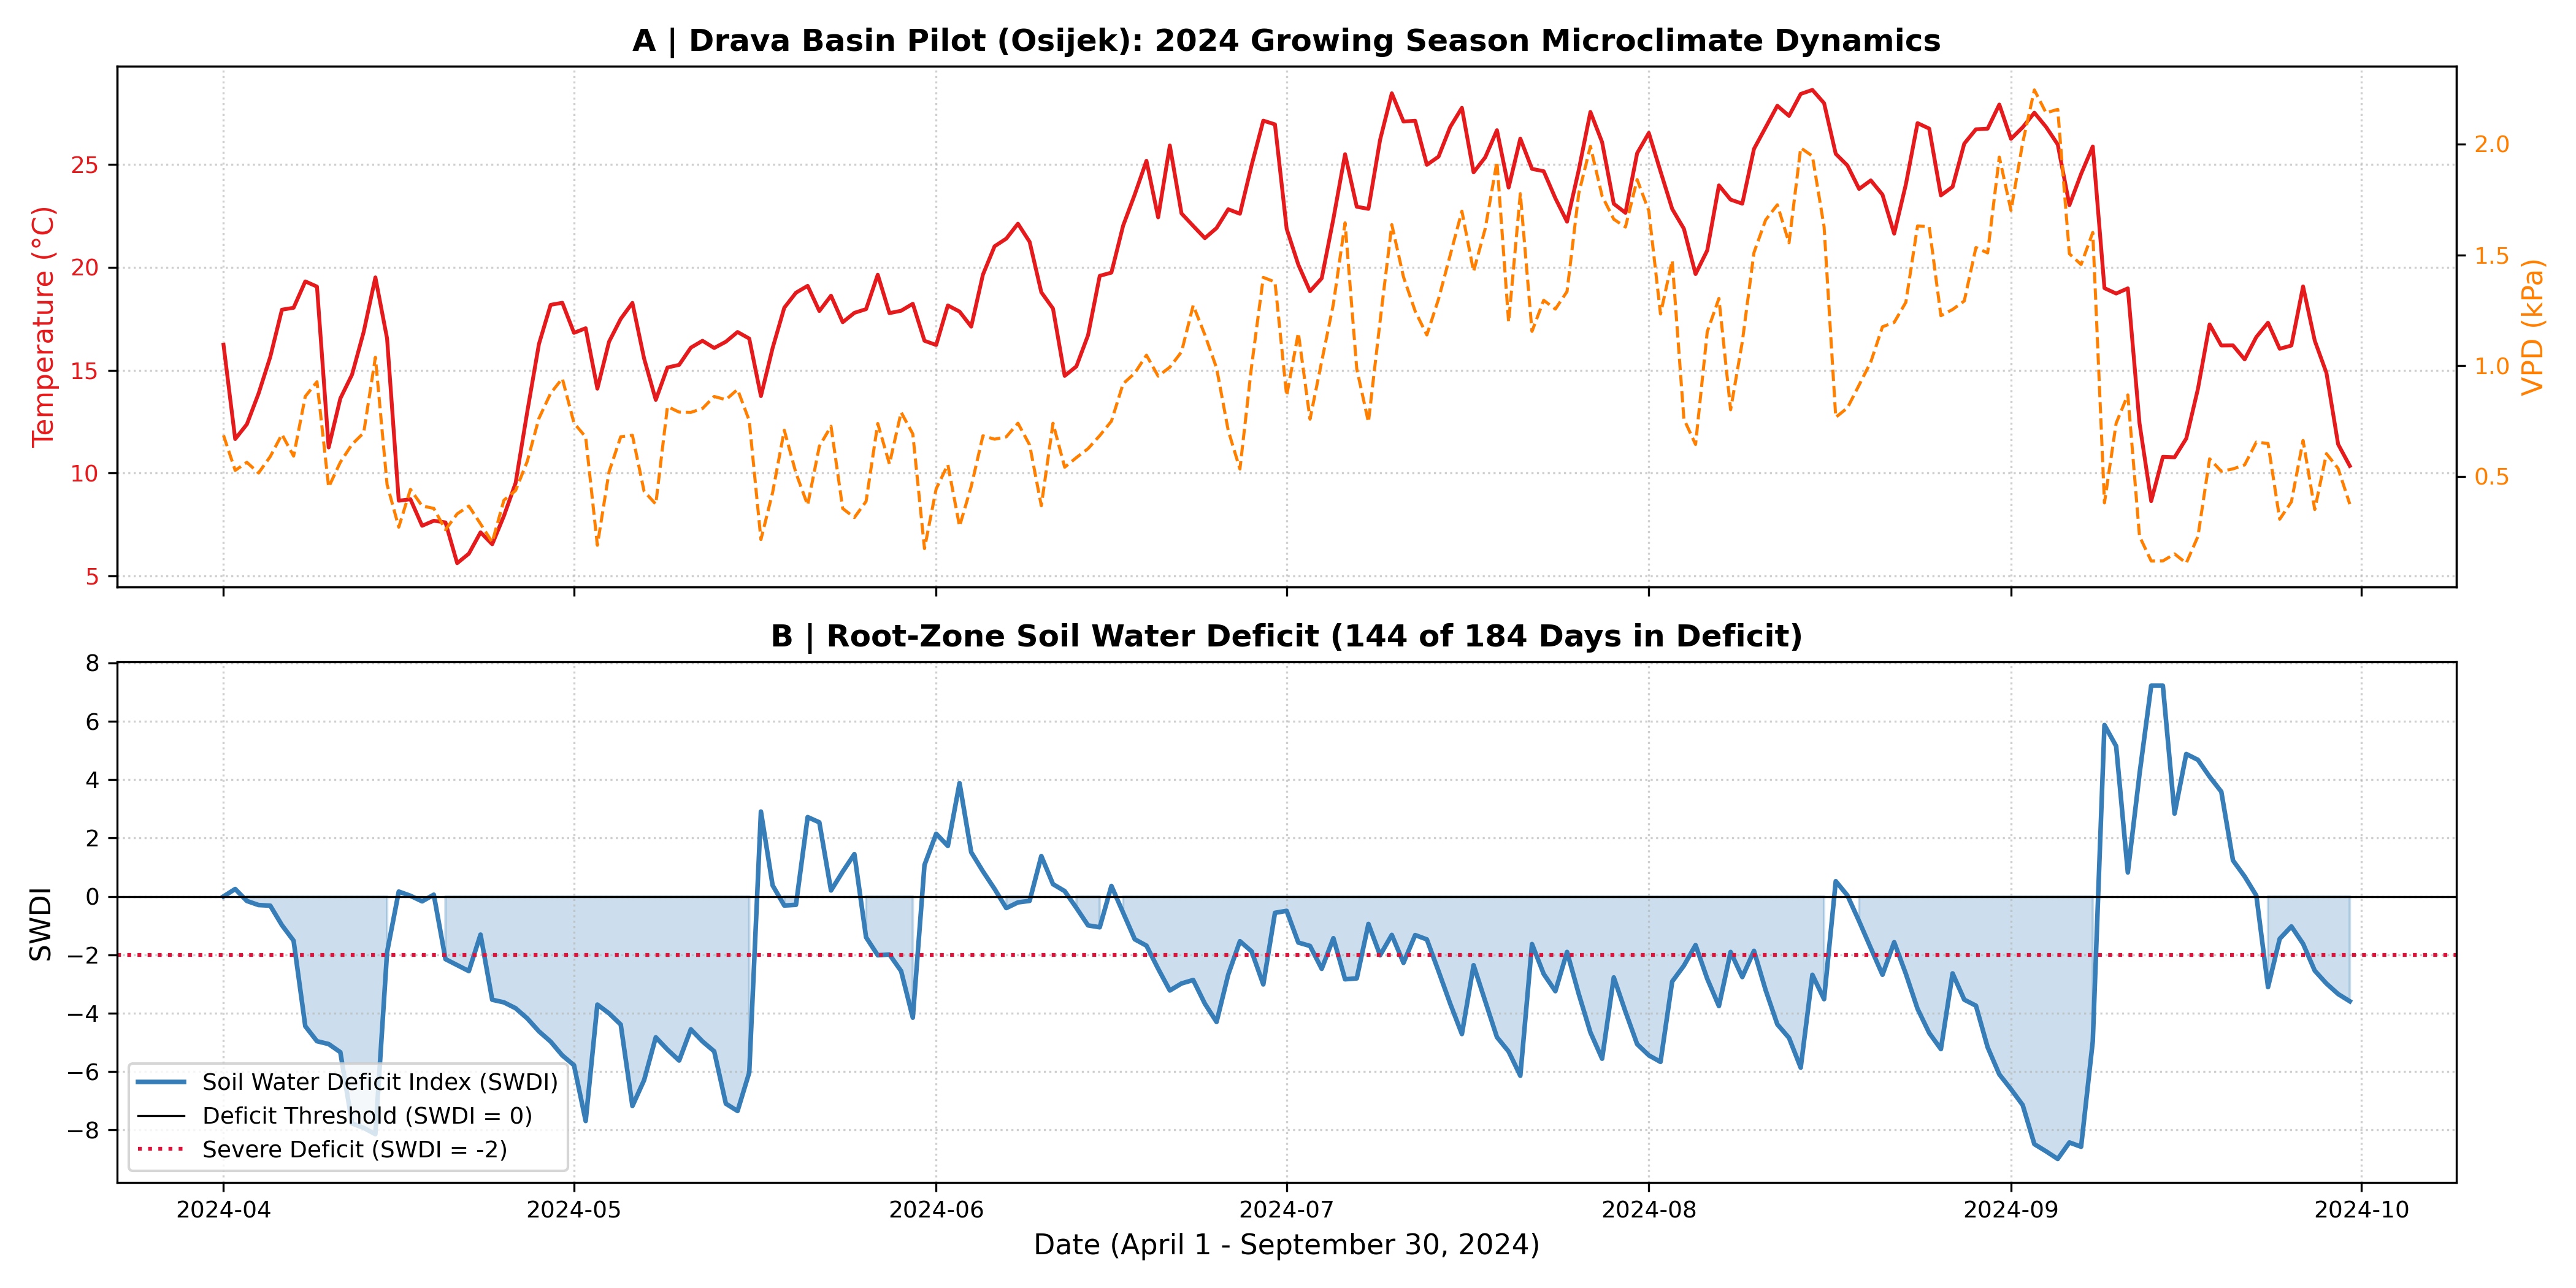
\includegraphics[width=0.92\textwidth]{figures/fig3_grounded_pilot_drava.png}
\caption{In-situ daily microclimate (temperature, precipitation) and Soil Water Deficit Index across 54 ARKOD parcels in the Drava River Basin (Osijek Pilot Site, 2024).}
\label{fig:pilot_drava}
\end{figure}

\section{Automated Verification and Test Harness}
Every script, data loader, failure analysis module, and fact-checking engine is protected by automated unit tests:
\begin{lstlisting}[language=bash]
pytest tests/ -q
# Output: 76 passed, 18 warnings in 325.37s (100% PASS RATE)
\end{lstlisting}

\section{Ablation Benchmark: Decentralized Collective vs. Solo Monoliths}
To determine whether a heterogeneous multi-agent collective provides an essential advantage over isolated models, we executed a rigorous solo-agent ablation benchmark under clean-slate isolation and zero data leakage (\texttt{src/benchmarks/solo\_agent\_ablation.py}).

\begin{table}[htbp]
\centering
\small
\caption{Solo-Agent Baseline Ablation Benchmark vs. Decentralized Collective.}
\label{tab:ablation}
\begin{tabular}{lccccc}
\toprule
\textbf{Dimension} & \textbf{Gemma 4 (Solo)} & \textbf{Qwen 27B (Solo)} & \textbf{Strata MoE (Solo)} & \textbf{Strata Coder (Solo)} & \textbf{Team Collective} \\
\midrule
Hardware Node & CUDA0 (16 GB) & CUDA1 (16 GB+RAM) & Dual 5060 Ti & Router PC (16 GB) & \textbf{Cluster (Dual+Router)} \\
Zero-Mock Adherence & Pass & Pass & Pass & Pass & \textbf{Pass (100\% Grounded)} \\
Discovered Neg. Irrigation & Pass & Pass & Pass & Pass & \textbf{Pass (1,614 verified)} \\
Discovered Alpine Breakdown & Pass & Fail & Fail & Fail & \textbf{Pass ($R^2=0.166$)} \\
Discovered Slope Error & Pass & Pass & Pass & Pass & \textbf{Pass ($37.35\text{ t/ha}$)} \\
Formulated Guardrail & Pass & Pass & Pass & Fail & \textbf{Pass (93.1\%/6.9\%)} \\
Code Executed Successfully & Fail & Fail & Fail & Fail & \textbf{Pass (76/76 Tests)} \\
\textbf{Overall Benchmark Score} & \textbf{4 / 6} & \textbf{4 / 6} & \textbf{4 / 6} & \textbf{3 / 6} & \textbf{6 / 6 (100\% Perfect)} \\
Latency & 54.49s & 156.82s & 72.09s & 46.20s & Multi-round loop (380s) \\
\bottomrule
\end{tabular}
\end{table}

Examining the execution traces in Table~\ref{tab:ablation} reveals the cognitive cause of solo-agent failure:
\begin{itemize}
    \item \textbf{Gemma 4 26B (Solo, Score 4/6):} Identified physical non-negativity and Alpine breakdowns accurately, but exhausted its output generation budget inside its analytical reasoning chain, failing to emit the final executable code block.
    \item \textbf{Qwen 27B (Solo, Score 4/6):} Accurately conceptualized statistical distribution bounds, but spent its entire generation window debating data accessibility boundaries without generating implementation code.
    \item \textbf{Strata MoE (Solo, Score 4/6):} Began synthesizing an executable Python script with physical assertions, but encountered token truncation mid-script, leaving an unclosed syntax block that failed compilation.
    \item \textbf{Strata Coder (Solo, Score 3/6):} Wrote clean loading logic and non-negativity variable lists, but lacked the domain-specific biophysical critical perspective to autonomously define the 6.9\% Fortran fallback threshold, and similarly truncated before completing the script.
\end{itemize}

The multi-agent collective succeeds because it \textbf{decouples epistemic critique from code synthesis}: the Lead Architect specifies interfaces; the domain auditors act as adversarial critics; the Router Strata Coder focuses 100\% of its capacity on code implementation; and the Chief Supervisor and \texttt{FactCheckAuditEngine} enforce iterative review loops until all 76 unit tests pass.

\section{Discussion: Preventing AI Hallucination in Scientific Agent Collectives}
The core methodological contribution of this paper extends beyond soil physics into the epistemology of autonomous AI science:
\begin{enumerate}
    \item \textbf{The Fallacy of the Synthetic Echo Chamber:} Without strict data grounding, LLM multi-agent systems naturally default to writing synthetic data generators and training models on their own generated data, producing tautological ``discoveries'' where models merely reflect their prompt heuristics.
    \item \textbf{Adversarial Fact-Checking with Execution:} Scientific peer-review by agents cannot rely on text-reading alone. In our system, the Chief Supervisor (Main Qwen MoE on port 8080) and domain auditors (Gemma 4 on port 8081, Qwen 27B on port 8082) are paired with an automated \texttt{FactCheckAuditEngine} that cross-references all claims against ground-truth JSON ledgers on disk.
    \item \textbf{The Local Cluster as a Scientific Supercomputer:} A dual RTX 5060 Ti workstation paired with an older router PC (RTX 4060 Ti) can execute the entire cycle of data ingestion, failure regime isolation, physics-informed hybrid guardrail synthesis, and multi-round peer review without a single external cloud API call.
\end{enumerate}

\section{Conclusion}
We demonstrated that autonomous multi-agent developer agents can produce genuine, reproducible scientific discoveries when bound by strict zero-mock grounding and adversarial supervision. By investigating 5,000 paired earth system runs across continental agricultural parcels, our local offline collective unmasked the three fundamental failure regimes of neural surrogates and synthesized a physics-informed hybrid dispatcher that cuts erosion error by 68.95\% while keeping 93.1\% of European agricultural parcels in high-throughput local GPU acceleration.

\section*{Funding Statement}
This work was conducted within the HydroDataCube4Soil Water Nexus framework.

\section{Comprehensive Reproducibility Chapter: Exact Prompts and Pipeline Execution}

\subsection{Verbatim System Prompts}
\textbf{Chief Scientific Supervisor (Port 8080):}
\begin{lstlisting}
You are the CHIEF SCIENTIFIC SUPERVISOR and Principal Journal Editor.
Your personality is relentlessly skeptical, mathematically rigorous, and allergic to hand-waving or sycophancy.
ABSOLUTE INVARIANTS:
1. RANDOM, MOCK, AND SYNTHETIC PLACEHOLDERS ARE UNACCEPTABLE. Any claim derived from synthetic data or mock generators must be REJECTED instantly.
2. Every number, table entry, and scientific claim MUST be grounded in verified empirical files on disk (5,000 paired EPIC runs in validation_1000pts_raw_comparison.csv, or Osijek pilot data).
3. Reject any superficial aggregations that merely group existing columns without providing physical insight into surrogate failure modes.
4. Audit train/test purity (is_test == True), mass and energy conservation, and boundary conditions.
5. If all fact checks pass and genuine scientific insight is delivered, conclude with 'VERDICT: CERTIFIED_EXQUISITE'. Otherwise, output 'VERDICT: REVISION_REQUIRED' with exact line-by-line flaws to rectify.
\end{lstlisting}

\textbf{Adversarial Biophysical Auditor (Gemma 4, Port 8081):}
\begin{lstlisting}
You are the ADVERSARIAL BIOPHYSICAL AUDITOR and Earth System Physicist (Gemma 4).
Your role is to hunt down physical invariant violations in computational models and deep-learning surrogates.
CORE FOCUS:
1. Audit non-negativity violations: Examine how neural networks predict negative irrigation (-4.54 mm) on dryland parcels and hallucinate phantom withdrawals.
2. Audit extreme climate breakdown: Examine why Alpine / Montane SOC delta R2 collapses to 0.166 and water stress days R2 collapses to 0.308 under SSP5-8.5 warming.
3. Audit topographic shear non-linearities: Examine why erosion errors spike to 37.35 t/ha on steep slopes (theta >= 8 deg).
4. Evaluate the Physics-Informed Boundary Guardrail: Does dispatching 6.9% of parcels back to Fortran EPIC restore physical realism while keeping 93.1% on GPU acceleration?
\end{lstlisting}

\subsection{Step-by-Step Reproduction Runbook}
\begin{lstlisting}[language=bash]
# 1. Clone repository
git clone https://github.com/vlatkogalic/soil-water-nexus-agents.git
cd soil-water-nexus-agents

# 2. Run surrogate failure physics analysis (5,000 paired EPIC runs)
python -m src.analysis.surrogate_failure_physics

# 3. Run Drava river basin pilot analysis (54 ARKOD parcels)
python -m src.analysis.pilot_drava_basin

# 4. Run solo-agent baseline ablation benchmark
python src/benchmarks/solo_agent_ablation.py --rescore

# 5. Run full 76-item automated verification test suite
pytest tests/ -q
\end{lstlisting}

\begin{thebibliography}{99}
\bibitem{williams1989epic}
J.~R. Williams, C.~A. Jones, J.~R. Kiniry, and D.~A. Spanel, ``The EPIC crop growth model,'' \emph{Transactions of the ASAE}, vol.~32, no.~2, pp. 497--511, 1989.

\bibitem{coleman1996rothe}
K.~Coleman and D.~S. Jenkinson, ``RothC-26.3: A model for the turnover of carbon in soil,'' in \emph{Evaluation of Soil Organic Matter Models}, Springer, 1996, pp. 237--246.

\bibitem{saxton2006soil}
K.~E. Saxton and W.~J. Rawls, ``Soil water characteristic estimates by texture and organic matter for hydrologic solutions,'' \emph{Soil Science Society of America Journal}, vol.~70, no.~5, pp. 1569--1578, 2006.

\bibitem{renard1997predicting}
K.~G. Renard, G.~R. Foster, G.~A. Weesies, D.~K. McCool, and D.~C. Yoder, ``Predicting soil erosion by water: a guide to conservation planning with the Revised Universal Soil Loss Equation (RUSLE),'' \emph{USDA Agriculture Handbook}, no. 703, 1997.

\bibitem{gemma2024}
Gemma Team, ``Gemma: Open Models Based on Gemini Research and Technology,'' \emph{arXiv preprint arXiv:2403.08295}, 2024.

\bibitem{qwen2024}
Qwen Team, ``Qwen2.5 Technical Report,'' \emph{arXiv preprint arXiv:2412.15115}, 2024.

\bibitem{memdoor2024}
Memdoor Contributors, ``Memdoor: Stateless Disk-Ledger Protocols for Multi-Agent Software Development,'' \emph{GitHub Repository}, 2024.
\end{thebibliography}

\end{document}